\section{Overview}
\label{sec:Overview}
Here we represents an overview of how the entire BBP architecture is composed of:

\begin{figure}[H]
    \begin{center}
        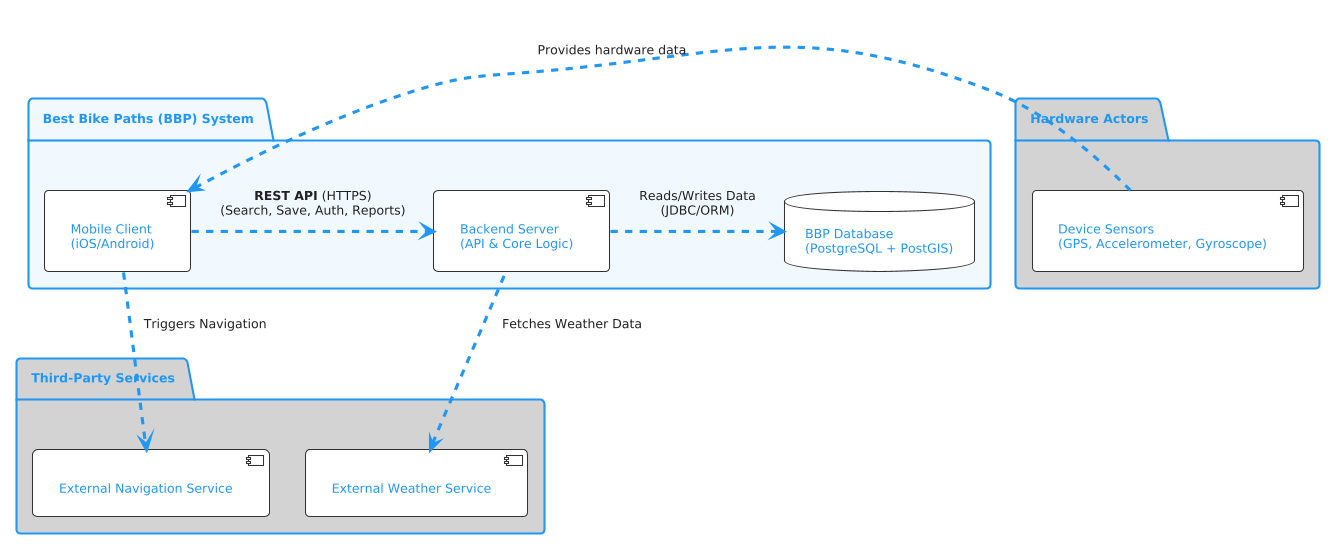
\includegraphics[width=1\linewidth]{DD/LaTeXCode/images/overview/overview.png}
        \caption{BBP Overview.}
        \label{fig:BBP_overview}%
    \end{center}
\end{figure}
\noindent Client Side:
\begin{itemize}
    \item \textbf{Mobile Client (iOS/Android):} Serves as the primary User Interface (UI) and data collection tool. It provides the native screens for all user interactions, runs a persistent foreground service to continuously capture data from device sensors (GPS, accelerometer, gyroscope), and manages the post-ride summary screen for reviewing events and setting visibility preferences.
\end{itemize}

\noindent Server Side:
\begin{itemize}
    \item \textbf{Backend Server (API \& Core Logic):} Handles all business logic, data integrity, and security via a secure REST API. It processes all incoming data from the client (e.g., saving new trips and paths atomically), manages user authentication, and performs complex server-side operations like aggregating trip statistics to update path averages. It is the single source of truth for all data.
    
    \item \textbf{BBP Database (PostgreSQL + PostGIS):} Stores all data related to users, paths, trips, and reports. It utilizes PostgreSQL for relational data and the \textbf{PostGIS} extension to efficiently store and query all geospatial data (e.g., path geometries, obstacle locations), enabling the core path-searching functionality.
    
    \item \textbf{Device Sensors (GPS, Accelerometer, Gyroscope):} Provides the raw hardware-level data streams to the Mobile Client. The GPS is used to build the trip's geometry, while the \textbf{Accelerometer} and \textbf{Gyroscope} provide motion data used to automatically detect potential obstacles (e.g., potholes).
    
    \item \textbf{External Weather Service:} Utilized by the Backend Server to fetch meteorological data. When a trip is saved, the server queries this API to retrieve weather conditions (e.g., temperature, wind speed) for the trip's time and location, adding valuable context to the user's log.
    
    \item \textbf{External Navigation Service:} Invoked by the Mobile Client to provide turn-by-turn directions. When a user "Follows Path," the client sends the route's destination or geometry to the device's default mapping application, allowing BBP to focus on its core recording and evaluation features.
\end{itemize}